\subsection{Hello Window}

Let's see if we can get GLFW up and running. First, create a \verb|.cpp| file and add the following includes to the top of your newly created file.

\begin{lstlisting}[language=C++]
    #include <glad/glad.h>
    #include <GLFW/glfw3.h>
\end{lstlisting}

Make sure to include \verb|glad.h| before \verb|glfw3.h|. Instead of \verb|glad.h| we can include \verb|GL/glew.h|. While for beginners \verb|glew| is sufficient, in more advanced use cases \verb|glad.h| might be more suitable.

Next, we create the \verb|main| function where we will instantiate the GLFW window:

\begin{lstlisting}[language=C++]
    int main()
    {
        glfwInit();
        glfwWindowHint(GLFW_CONTEXT_VERSION_MAJOR, 3);
        glfwWindowHint(GLFW_CONTEXT_VERSION_MINOR, 3);
        glfwWindowHint(GLFW_OPENGL_PROFILE, GLFW_OPENGL_CORE_PROFILE);
        //glfwWindowHint(GLFW_OPENGL_FORWARD_COMPAT, GL_TRUE);
    
        return 0;
    }
\end{lstlisting}

\verb|glfwWindowHint(GLFW_CONTEXT_VERSION_MAJOR, 3);| \\ and \verb|glfwWindowHint(GLFW_CONTEXT_VERSION_MINOR, 3);| translates to setting the OpenGL version to 3.3. The next line sets the OpenGL profile to the core profile. The core profile means that deprecated functionality will be removed. Note that on Mac OS X you need to add \\ \verb|glfwWindowHint(GLFW_OPENGL_FORWARD_COMPAT, GL_TRUE);| to your initialization code for it to work.

Next we're required to create a window object. This window object holds all the windowing data and is required by most of GLFW's other functions.

\begin{lstlisting}[language=C++]
    GLFWwindow* window = glfwCreateWindow(800, 600, "LearnOpenGL", NULL, NULL);
    if (window == NULL)
    {
        std::cout << "Failed to create GLFW window" << std::endl;
        glfwTerminate();
        return -1;
    }
    glfwMakeContextCurrent(window);
\end{lstlisting}

The \verb|glfwCreateWindow| function requires the window width and height as its first two arguments respectively. The third argument allows us to create a name for the window; for now we call it "LearnOpenGL" but you're allowed to name it however you like. We can ignore the last 2 parameters. The function returns a \verb|GLFWwindow| object that we'll later need for other GLFW operations. After that we tell GLFW to make the context of our window the main context on the current thread.

We will also need to initialize GLAD as seen below:

\begin{lstlisting}[language=C++]
    if (!gladLoadGLLoader((GLADloadproc)glfwGetProcAddress))
    {
        std::cout << "Failed to initialize GLAD" << std::endl;
        return -1;
    }    
\end{lstlisting}

We pass GLAD the function to load the address of the OpenGL function pointers which is OS-specific. GLFW gives us \verb|glfwGetProcAddress| that defines the correct function based on which OS we're compiling for.

Before we can start rendering we have to do one last thing. We have to tell OpenGL the size of the rendering window so OpenGL knows how we want to display the data and coordinates with respect to the window. We can set those dimensions via the glViewport function:

\begin{lstlisting}[language=C++]
    glViewport(0, 0, 800, 600);
\end{lstlisting}

The first two parameters of \verb|glViewport| set the location of the lower left corner of the window. The third and fourth parameter set the width and height of the rendering window in pixels, which we set equal to GLFW's window size.

We could actually set the viewport dimensions at values smaller than GLFW's dimensions; then all the OpenGL rendering would be displayed in a smaller window and we could for example display other elements outside the OpenGL viewport.

\newpage

\begin{note}
    Behind the scenes OpenGL uses the data specified via \verb|glViewport| to transform the 2D coordinates it processed to coordinates on your screen. For example, a processed point of location (-0.5,0.5) would (as its final transformation) be mapped to (200,450) in screen coordinates. Note that processed coordinates in OpenGL are between -1 and 1 so we effectively map from the range (-1 to 1) to (0, 800) and (0, 600).
\end{note}

However, the moment a user resizes the window the viewport should be adjusted as well. We can register a callback function on the window that gets called each time the window is resized. This resize callback function has the following prototype:

\begin{lstlisting}[language=C++]
    void framebuffer_size_callback(GLFWwindow* window, int width, int height); 
\end{lstlisting}

The framebuffer size function takes a \verb|GLFWwindow| as its first argument and two integers indicating the new window dimensions. Whenever the window changes in size, GLFW calls this function and fills in the proper arguments for you to process.

\begin{lstlisting}[language=C++]
    void framebuffer_size_callback(GLFWwindow* window, int width, int height)
    {
        glViewport(0, 0, width, height);
    }  
\end{lstlisting}

We do have to tell GLFW we want to call this function on every window resize by registering it:

\begin{lstlisting}[language=C++]
    glfwSetFramebufferSizeCallback(window, framebuffer_size_callback); 
\end{lstlisting}

When the window is first displayed \verb|framebuffer_size_callback| gets called as well with the resulting window dimensions. For retina displays width and height will end up significantly higher than the original input values.

There are many callbacks functions we can set to register our own functions. For example, we can make a callback function to process joystick input changes, process error messages etc. We register the callback functions after we've created the window and before the render loop is initiated.

We don't want the application to draw a single image and then immediately quit and close the window. We want the application to keep drawing images and handling user input until the program has been explicitly told to stop. For this reason we have to create a while loop, that we now call the \blue{render} loop, that keeps on running until we tell GLFW to stop. The following code shows a very simple render loop:

\begin{lstlisting}[language=C++]
    while(!glfwWindowShouldClose(window))
    {
        glfwSwapBuffers(window);
        glfwPollEvents();    
    }
\end{lstlisting}

\newpage

\begin{important}
    The \verb|glfwWindowShouldClose| function checks at the start of each loop iteration if GLFW has been instructed to close. If so, the function returns true and the render loop stops running, after which we can close the application.
    The \verb|glfwPollEvents| function checks if any events are triggered (like keyboard input or mouse movement events), updates the window state, and calls the corresponding functions (which we can register via callback methods). The \verb|glfwSwapBuffers| will swap the color buffer (a large 2D buffer that contains color values for each pixel in GLFW's window) that is used to render to during this render iteration and show it as output to the screen.
\end{important}

\begin{note}
    \begin{center}
        \textbf{Double Buffer}
    \end{center}
    When an application draws in a single buffer the resulting image may display flickering issues. This is because the resulting output image is not drawn in an instant, but drawn pixel by pixel and usually from left to right and top to bottom. Because this image is not displayed at an instant to the user while still being rendered to, the result may contain artifacts. To circumvent these issues, windowing applications apply a double buffer for rendering. The \textbf{front} buffer contains the final output image that is shown at the screen, while all the rendering commands draw to the \textbf{back} buffer. As soon as all the rendering commands are finished we swap the back buffer to the front buffer so the image can be displayed without still being rendered to, removing all the aforementioned artifacts.
\end{note}

As soon as we exit the render loop we would like to properly clean/delete all of GLFW's resources that were allocated. We can do this via the \verb|glfwTerminate| function that we call at the end of the main function.

\begin{lstlisting}[language=C++]
    glfwTerminate();
    return 0;
\end{lstlisting}

This will clean up all the resources and properly exit the application. Now try to compile your application and if everything went well you should see the following output:

\begin{center}
    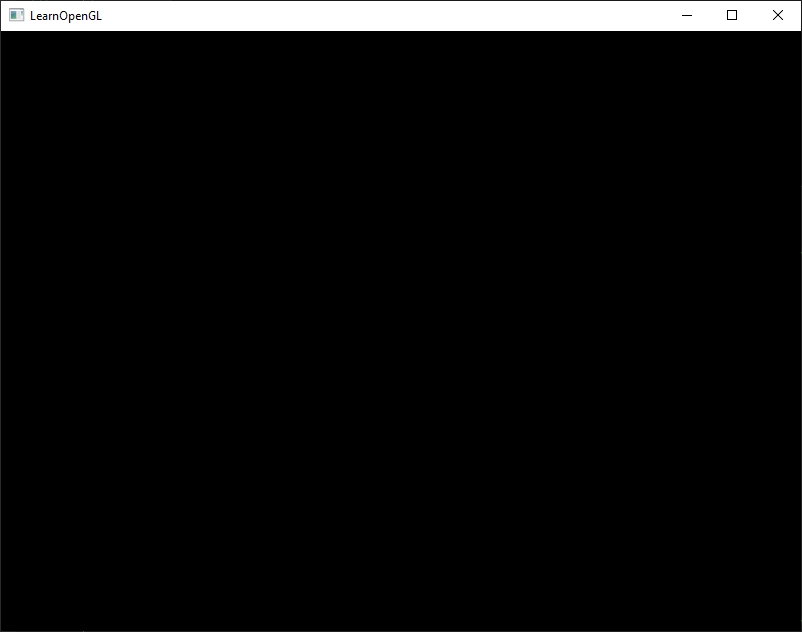
\includegraphics[scale=0.4]{pics/hellowindow.png}
\end{center}

We also want to have some form of \textbf{input} control in GLFW and we can achieve this with several of GLFW's input functions. We'll be using GLFW's \verb|glfwGetKey| function that takes the window as input together with a key. The function returns whether this key is currently being pressed. We're creating a processInput function to keep all input code organized:

\begin{lstlisting}[language=C++]
    void processInput(GLFWwindow *window)
    {
        if(glfwGetKey(window, GLFW_KEY_ESCAPE) == GLFW_PRESS)
            glfwSetWindowShouldClose(window, true);
    }
\end{lstlisting}

Here we check whether the user has pressed the escape key (if it's not pressed, \verb|glfwGetKey| returns \verb|GLFW_RELEASE|). If the user did press the escape key, we close GLFW by setting its WindowShouldClose property to true using \verb|glfwSetwindowShouldClose|. The next condition check of the main while loop will then fail and the application closes.

We then call processInput every iteration of the render loop:

\begin{lstlisting}[language=C++]
    while (!glfwWindowShouldClose(window))
    {
        processInput(window);

        glfwSwapBuffers(window);
        glfwPollEvents();
    }  
\end{lstlisting}

This gives us an easy way to check for specific key presses and react accordingly every frame. An iteration of the render loop is more commonly called a \blue{frame}.

We want to place all the rendering commands in the render loop, since we want to execute all the rendering commands each iteration or frame of the loop. This would look a bit like this:

\begin{lstlisting}[language=C++]
    // render loop
    while(!glfwWindowShouldClose(window))
    {
        // input
        processInput(window);

        // rendering commands here
        ...

        // check and call events and swap the buffers
        glfwPollEvents();
        glfwSwapBuffers(window);
    }
\end{lstlisting}

Just to test if things actually work we want to clear the screen with a color of our choice. At the start of frame we want to clear the screen. Otherwise we would still see the results from the previous frame (this could be the effect you're looking for, but usually you don't). We can clear the screen's color buffer using glClear where we pass in buffer bits to specify which buffer we would like to clear. The possible bits we can set are \verb|GL_COLOR_BUFFER_BIT|, \verb|GL_DEPTH_BUFFER_BIT| and \verb|GL_STENCIL_BUFFER_BIT|. Right now we only care about the color values so we only clear the color buffer.

\begin{lstlisting}[language=C++]
    glClearColor(0.2f, 0.3f, 0.3f, 1.0f);
    glClear(GL_COLOR_BUFFER_BIT);
\end{lstlisting}

Note that we also specify the color to clear the screen with using \verb|glClearColor|. Whenever we call glClear and clear the color buffer, the entire color buffer will be filled with the color as configured by \verb|glClearColor|. This will result in a dark green-blueish color.

\begin{center}
    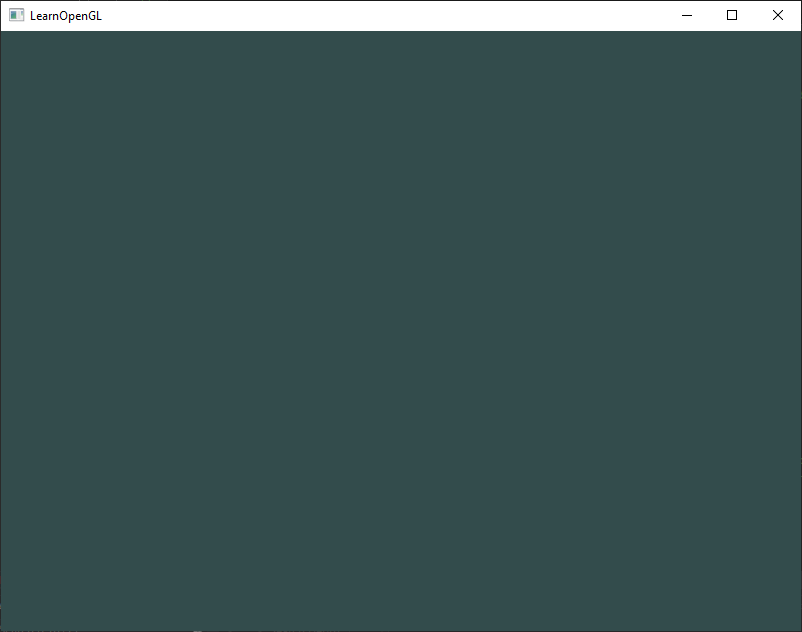
\includegraphics[scale=0.4]{pics/hellowindow2.png}
\end{center}